\input texbase

\titulo{Exercício Programa 2}
\materia{MAC5915 - Laboratório de Visão Computacional e Processamento de Imagens}

\aluno{Fernando Omar Aluani}{6797226}

\begin{document}
\cabecalho

%===================================================================================

\section{Funcionamento do Algoritmo}
Nessa seção irei explicar como funciona o algoritmo de categorização visual usando 
\textit{bags of keypoints} que implementei, baseado na descrição desse algoritmo no
artigo contido no PACA. Dividi ele em duas grandes partes,
treinamento e testes, e cada uma trata de uma parte do \textit{dataset}.

%----------------------------------------------------------------------
\subsection{Treinamento}
O treinamento é a primeira parte do algoritmo a ser executada. Ele retira um conjunto
de imagens de cada classe do dataset e usa essas imagens para o treinamento. Isso se dá em algumas etapas, em ordem:

\subsubsection{Calcula Keypoints}
Primeiramente, o programa calcula os keypoints (descritores) de cada imagem de treinamento. A qual classe
elas pertencem não importa nessa etapa. Ele pode usar SIFT ou SURF para isso. Os descritores são
vetores (128-dimensional no caso do SIFT) de números.

\subsubsection{Clusterização}
Após calcular os keypoints, o programa usa o algoritmo de KMEANS para clusterizar os keypoints
em K clusters (por padrão, 1000). Essa é a etapa que usualmente leva mais tempo para ser executada,
e ela gera os pontos que identificam os clusters: os pontos centrais deles. Cada um desses pontos tem
a mesma dimensão dos keypoints.

\subsubsection{Criação do Vocabulário}
A terceira etapa cria o ``vocabulário'', que iremos usar nas próximas etapas. Ele consiste em um
classificador K-NEAREST-NEIGHBOUR (KNN), treinado com os centros dos clusters, sendo que cada
centro recebe um rótulo diferente.

\subsubsection{Calcula Histogramas}
Para cada imagem de treinamento o algoritmo recalcula os descritores, e com a ajuda do KNN do vocabulário,
descobre quais são os clusters em que os descritores estão mais próximos. Com isso ele constrói um
histograma para cada imagem que diz em quais clusters os descritores ``cairam''.

\subsubsection{treina classificador com histogramas}
Finalmente, o programa usa os histogramas calculados anteriormente, e os dados de para qual 
classe do dataset cada um deles pertence, e usa isso para treinar um classificador, que pode
ser KNN ou Support Vector Machines (SVM). Este é o classificador que categoriza imagens, e será
usado nos testes.

%----------------------------------------------------------------------
\subsection{Testes}
Depois da etapa de treinamento, as imagens do dataset (ou um subconjunto delas) que sobraram 
são usadas para testes. Essa parte é bem simples: para cada imagem de teste, seu histograma
é calculado e passado para o classificador para obter sua classificação. Comparo a resposta
do classificador com a classe real da imagem e então o programa mostra a porcentagem de
acerto do classificador em cada classe.

%===================================================================================
\section{Implementação}
Eu implementei o algoritmo em \emph{Python}, na forma de um script que pode ser executado
como um programa na linha de comando ou importado por outro script como uma biblioteca.

Algoritmos já conhecidos como KMEANS, SIFT, SURF, KNN e SVM eu usei implementações prontas
da biblioteca \emph{OpenCV}.

\subsection{Dataset}
O programa assume que o dataset é passado de um jeito bem específico para ele: como o caminho para
uma pasta onde estão contidas TODAS imagens do dataset. Note que a pasta do dataset 
deve conter todas imagens nela - subpastas contidas dentro do dataset serão ignoradas ou 
poderão dar erro no script (não testei esse caso).

Outra suposição que ele faz com o dataset é que todas imagens são salvas em formato \emph{.jpg},
seguindo o seguinte formato de nomeação:
\begin{verbatim}
     <nome_da_classe>_<indice>.jpg
\end{verbatim}
Exemplos: 
\begin{verbatim}
classe_A_1.jpg, classe_A_2.jpg, algum_nome_de_classe_10.jpg...
\end{verbatim}

Isso se deve a minha escolha de deixar esse aspecto do programa mais voltado ao dataset
que usei para testar.

\subsubsection{Divisão do Dataset}
Outro fato importante é como ele divide as imagens do dataset para treinamento e testes.
Por padrão, ele ordena as imagens de cada classe de acordo com seus índices, e então usa as 
primeiras \textbf{X\%} imagens de cada classe como treinamento, onde X é um parametro passado pelo usuário.

Também é possível, por meio de outro paramêtro, que ele busque as imagens de treinamento aleatoriamente.
Nesse caso, ele ainda separa X\% imagens de cada classe para treinamento, mas em vez de pegar as
primeiras, o programa pega elas aleatoriamente dentre as imagens da classe.

Para o teste, são escolhidas \textbf{N} imagens de cada classe aleatóriamente, dentre as imagens que
sobraram depois do treinamento. Uma imagem nunca será escolhida para treinamento e teste simultaneamente,
e também nunca será escolhida duas vezes para a mesma etapa.

%----------------------------------------------------------------------
\subsection{Execução}
Para executar o script é necessário Python versão $2.7$ ou mais (mas não versão 3 ou mais),
OpenCV (para python) e a biblioteca de python \emph{NumPy} instaladas. Essas bibliotecas são
fáceis de encontrar e instalar em diversas plataformas.

Com tudo necessário instalado, para rodar o script basta executá-lo na linha de comando.
Passando o parametro \textbf{--help} irá mostrar a ajuda do programa, listando todos 
parametros possíveis, o que eles fazem e valores padrão.

%===================================================================================
\section{Resultados}
Aqui irei mostrar alguns dos resultados do programa. O dataset que usei foi um de
animais de estimação\footnote{
Seguindo uma indicação do artigo, peguei esse dataset em http://www.robots.ox.ac.uk/~vgg/data/pets/.
Ele continha originalmente 37 classes de animais. Eu removi várias classes para simplificar o dataset
para meus testes.
} que contém 10 classes de animais (raças de cachorros),
sendo que cada classe tem aproximadamente 200 imagens coloridas com resoluções entre
200 e 500 pixels em cada eixo. Cada classe tem o nome da raça do cachorro, mas por simplicidade 
também irei me referir a elas nas próximas páginas por uma letra de A a J, como será mostrado na seção \emph{Tempos de execução}.

Nos testes usei esse dataset em duas formas:
\begin{enumerate}
  \item \textbf{Dataset Total}: Ele completo (as 10 classes).
  \item \textbf{Mini Dataset}: um subconjunto de 3 das 10 classes do dataset. Ainda com as mesmas imagens.
\end{enumerate}

No total, rodei 6 testes:
\begin{enumerate}
  \item \textbf{KNN}: Com o dataset total, usando KNN como classificador e SURF como extrator. 40\% das
    imagens de cada classe como treinamento (80 imagens de cada classe) e testando com 80 imagens em cada classe.
  \item \textbf{SVM}: O mesmo que o teste acima, mas com o classificador SVM.
  \item \textbf{KNN\_sift\_tp05}: Com o mini dataset, usando o KNN como classificador e SIFT como extrator.
    50\% das imagens de cada classe para treinamento (100 imagens de cada classe) e testando com 80
    imagens de cada classe.
  \item \textbf{KNN\_surf\_tp05}: Mesmo que o teste acima, mas com SURF como extrator.
  \item \textbf{SVM\_sift\_tp05}: Mesmo que o teste acima, mas com classificador SVM e extrator SIFT.
  \item \textbf{SVM\_surf\_tp05}: Mesmo que o teste acima, mas com extrator SURF.
\end{enumerate}

Todos os testes foram executados na mesma máquina, e como não usei a opção para usar imagens aleatórias 
para treinamento, eles usaram as mesmas imagens para o treinamento. Note que os testes
que usaram 50\% de imagens para treinamento usaram as mesmas 40\% dos outros dois testes, e 10\% a mais.
Todos testes usaram o valor padrão do número de clusters K: 1000.

\begin{figure}
  \centering
  \begin{subfigure}[b]{0.4\textwidth}
    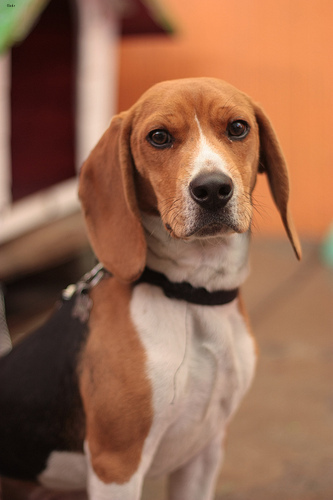
\includegraphics[width=\textwidth]{beagle_good.jpg}
    \caption{Um \textit{beagle} (F) }
  \end{subfigure}
  ~ 
  \begin{subfigure}[b]{0.4\textwidth}
    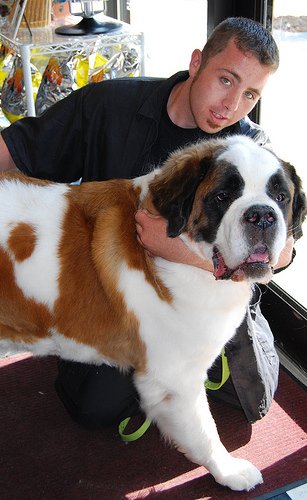
\includegraphics[width=\textwidth]{saint_bernard_good.jpg}
    \caption{Um \textit{saint bernard} (E)}
  \end{subfigure}
  \caption{Exemplos de imagens que foram corretamente classificadas em todos testes.}
  \label{fig:perfectgood}
\end{figure}

\begin{figure}
  \centering
  \begin{subfigure}[b]{0.4\textwidth}
    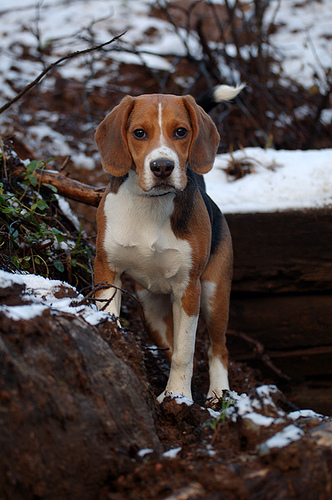
\includegraphics[width=\textwidth]{beagle_bad.jpg}
    \caption{Um \textit{beagle} (F), classificado como \textit{saint bernard} em 3 testes. }
  \end{subfigure}
  ~ 
  \begin{subfigure}[b]{0.4\textwidth}
    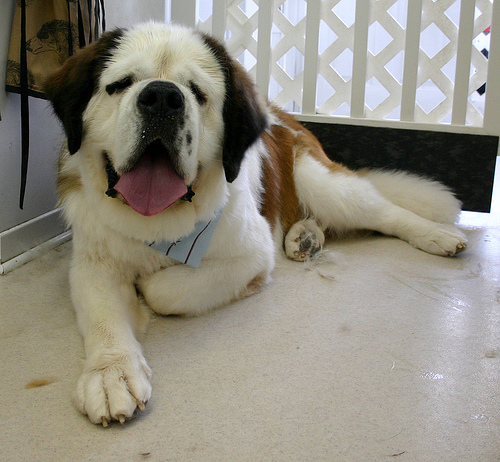
\includegraphics[width=\textwidth]{saint_bernard_bad.jpg}
    \caption{Um \textit{saint bernard} (E), classificado como \textit{beagle} em 5 testes. }
  \end{subfigure}
  \caption{Exemplos de imagens que foram incorretamente classificadas em todos testes.}
  \label{fig:perfectbad}
\end{figure}


\begin{figure}
  \centering
  \begin{subfigure}[b]{0.6\textwidth}
    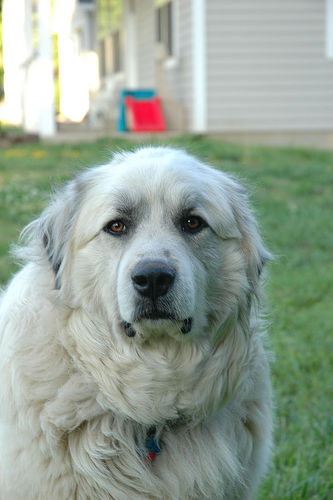
\includegraphics[width=\textwidth]{great_pyrenees.jpg}
  \end{subfigure}
  \caption{Um \textit{great pyrenees} (E), classificado corretamente nos dois testes com dataset mini e SURF, e incorretamente
      como \textit{saint bernard} nos dois testes com dataset mini e SIFT.}
  \label{fig:pyrenees}
\end{figure}

Também notei que, com exceção da classe \textit{great pyrenees} (I), todas as classes tiveram algumas poucas
imagens que foram corretamente classificadas em todos testes, como as mostradas na figura \ref{fig:perfectgood}.
Por outro lado, todas classes tiveram várias imagens que foram incorretamente classificadas em todos testes, tendo
alguns exemplos na figura \ref{fig:perfectbad}. Como
dos seis testes só dois deles testaram com as 10 classes, os exemplos de imagem que mostrarei são das 3 classes
que foram usadas em todos testes pois elas são mais representativas. 

Outro exemplo curioso é o da figura \ref{fig:pyrenees}. Essa imagem foi corretamente classificada nos dois testes
com dataset mini e extrator SURF, mas foi incorretamente classificada como \textit{saint bernard} nos dois testes
com dataset mini e extrator SIFT. No teste com dataset total e classificador KNN ela foi incorretamente classificada 
como \textit{english cocker spaniel}, enquanto que no teste com dataset total e classificador SVM ela não foi usada.

\subsection{Tempos de execução}
A tabela a seguir mostra o tempo de execução das diversas partes do algoritmo e a
precisão geral dele para cada um dos testes. As colunas são:
\begin{itemize}
  \item \textbf{Classes}: Número de classes contidas nesse teste.
  \item \textbf{Descs}: Tempo total que levou para calcular os descritores das imagens de treinamento, em segundos.
  \item \textbf{KMeans}: Tempo que levou para executar o KMeans e clusterizar os descritores, em segundos.
  \item \textbf{Hists}: Tempo total que levou para calcular os histogramas das imagens de treinamento, em segundos.
  \item \textbf{Treino}: Tempo que levou para executar o treinamento do algoritmo, em segundos.
  \item \textbf{Testes}: Tempo que levou para rodar os testes, em segundos.
  \item \textbf{Total}: Tempo total de execução do programa, em segundos.
  \item \textbf{AT}: Porcentagem geral de acertos dos testes (juntando todos os testes, de todas classes).
\end{itemize}
\begin{tabular}{ | l | c | c | c | c | c | c | c | r | }
\hline
Teste       & Classes & Descs & KMeans & Hists & Treino & Testes & Total & AT \\
\hline
KNN & 10 & 109.11s & 1318.07s & 218.04s & 1645.69s & 188.11s & 1833.81s & 17.5\% \\
\hline
KNN\_sift\_tp05 & 3 & 84.27s & 1311.64s & 126.02s & 1522.08s & 86.05s & 1608.13s & 42.1\% \\
\hline
KNN\_surf\_tp05 & 3 & 33.23s & 380.49s & 65.73s & 479.51s & 46.93s & 526.45s & 48.8\% \\
\hline
SVM & 10 & 99.11s & 1373.76s & 259.89s & 1734.20s & 180.24s & 1914.45s & 26.0\% \\
\hline
SVM\_sift\_tp05 & 3 & 80.95s & 1169.20s & 112.32s & 1362.74s & 75.49s & 1438.25s & 52.1\% \\
\hline
SVM\_surf\_tp05 & 3 & 33.07s & 369.74s & 60.67s & 463.66s & 45.56s & 509.22s & 53.3\% \\
\hline
\end{tabular}

\vspace{10pt}
A tabela a seguir mostra a taxa de acerto de cada teste para cada classe. As classes
estão indicadas como letras de A a J, que indicam, respectivamente, as classes 
\textit{leonberger}, \textit{english setter}, \textit{pug}, \textit{basset hound}, \textit{saint bernard},
\textit{beagle}, \textit{shiba inu}, \textit{english cocker spaniel}, \textit{great pyrenees}, \textit{newfoundland}.\\
\begin{tabular}{ | l | c | c | c | c | c | c | c | c | c | c | }
\hline
Teste       & A & B & C & D & E & F & G & H & I & J \\
\hline
KNN & 8.8\% & 15.0\% & 8.8\% & 11.2\% & 26.2\% & 15.0\% & 17.5\% & 27.5\% & 35.0\% & 10.0\% \\
\hline
KNN\_sift\_tp05 & -- & -- & -- & -- & 50.0\% & 50.0\% & -- & -- & 26.2\% & -- \\
\hline
KNN\_surf\_tp05 & -- & -- & -- & -- & 48.8\% & 48.8\% & -- & -- & 48.8\% & -- \\
\hline
SVM & 27.5\% & 28.8\% & 31.2\% & 22.5\% & 25.0\% & 23.8\% & 22.5\% & 25.0\% & 28.8\% & 25.0\% \\
\hline
SVM\_sift\_tp05 & -- & -- & -- & -- & 56.2\% & 57.5\% & -- & -- & 42.5\% & -- \\
\hline
SVM\_surf\_tp05 & -- & -- & -- & -- & 56.2\% & 51.2\% & -- & -- & 52.5\% & -- \\
\hline
\end{tabular}


\subsection{Conclusões}
Achei que o algoritmo é simples de implementar assim como o artigo diz, mesmo sendo que
no começo tive dificuldade em entender como gerar os histogramas para treinar o algoritmo...

Em relação à eficiência do algoritmo, também achei de acordo com o que o artigo diz. Mas depende
da escolha de classificador, extrator, e implementação do OpenCV. A implementação do OpenCV que
usei tinha suporte a execução \textit{multi-thread} das classes e funções que usei (kmeans, classificadores
e extratores). Isso acelerou bastante a execução do programa em relação a testes anteriores que fiz.

Entre os classificadores KNN e SVM, o SVM aparenta ser um pouco mais rápido que o KNN, e definitivamente
apresenta resultados mais precisos. Quanto aos extratores, o SURF não só é bem mais rápido que o SIFT,
como também apresenta resultados melhores. Podemos ver essa diferença notável de velocidade entre os testes
com dataset total e os com mini dataset com extrator SIFT. Os com dataset total estão usando 800 imagens 
para treinamento, enquanto os com o mini estão usando 300, e ainda assim a diferença de tempo deles é pequena.
Esses mesmos com SIFT e mini dataset levam quase três vezes mais que os com SURF.

No geral, esperava que a precisão do algoritmo fosse melhor... Também estranhei a queda de precisão para os testes
com mais classes. Acredito que nesses a perda de precisão se deve mais ao fato de ter 7 classes a mais do que 20
imagens a menos para treinar cada classe. 

Porém não posso afirmar com certeza que implementei o algoritmo exatamente como deveria ser para alcançar uma 
precisão alta, ou que usei os paramêtros certos. Como também só testei com o mesmo dataset, não tenho como saber
se esse dataset especificamente apresenta um desafio maior para o algoritmo de categorização visual.


\end{document}
